\section{Cálculo Multivariado}

	\subsection{O Espaço n-Dimensional ($\mathbb{R}^{n}$)}

		\begin{longtable}{
		@{}
		C{1\textwidth} 
		@{}}

			\toprule
			%------------------------------
			\textbf{Equações em $\mathbb{R}^{2}$} (linha) e $\mathbb{R}^{3}$ (plano)
			%------------------------------
			\tabularnewline
			\midrule
			%------------------------------
			{\large \begin{tabular}[c]{@{}c@{}}

				Para $\mathbb{R}^{2}$ \\
				
				$ax + by + c = 0$ (com $a$ e $b$ reais e $a$ e $b$ não nulos simultaneamente) \\

				Para $\mathbb{R}^{3}$ \\
				
				$ax + by + cz + d = 0$ (com $a, b, c, d$ reais e $a, b, c$ não nulos simultaneamente)

			\end{tabular}}
			%------------------------------
			\tabularnewline
			\midrule
			%------------------------------
			\textbf{Equação do Círculo}
			%------------------------------
			\tabularnewline
			\midrule
			%------------------------------
			{\large $(x - a)^{2} + (y - b)^{2} = r^{2}$}
			%------------------------------
			\tabularnewline
			\midrule
			%------------------------------
			\textbf{Distância entre dois Pontos}
			%------------------------------
			\tabularnewline
			\midrule
			%------------------------------
			{\large \begin{tabular}[c]{@{}c@{}}

				Para $\mathbb{R}^{2}$ \hspace{1cm} $d(P_{1}, P_{2}) = \sqrt{(x_{2} - x_{1})^{2} + (y_{2} - y_{1})^{2}}$ \\

				Para $\mathbb{R}^{3}$ \hspace{1cm} $d(P_{1}, P_{2}) = \sqrt{(x_{2} - x_{1})^{2} + (y_{2} - y_{1})^{2} + (z_{2} - z_{1})^{2}}$ \\

				Para $\mathbb{R}^{n}$ \hspace{1cm} $d(P_{1}, P_{2}) = \sqrt{(y_{1} - x_{1})^{2} + (y_{2} - x_{2})^{2} + \dots + (y_{n} - x_{n})^{2}}$

			\end{tabular}}
			%------------------------------
			\tabularnewline
			\midrule
			%------------------------------
			\textbf{Planos Coordenados}
			%------------------------------
			\tabularnewline
			\midrule
			%------------------------------
			\begin{figure}[H]
			    \centering
				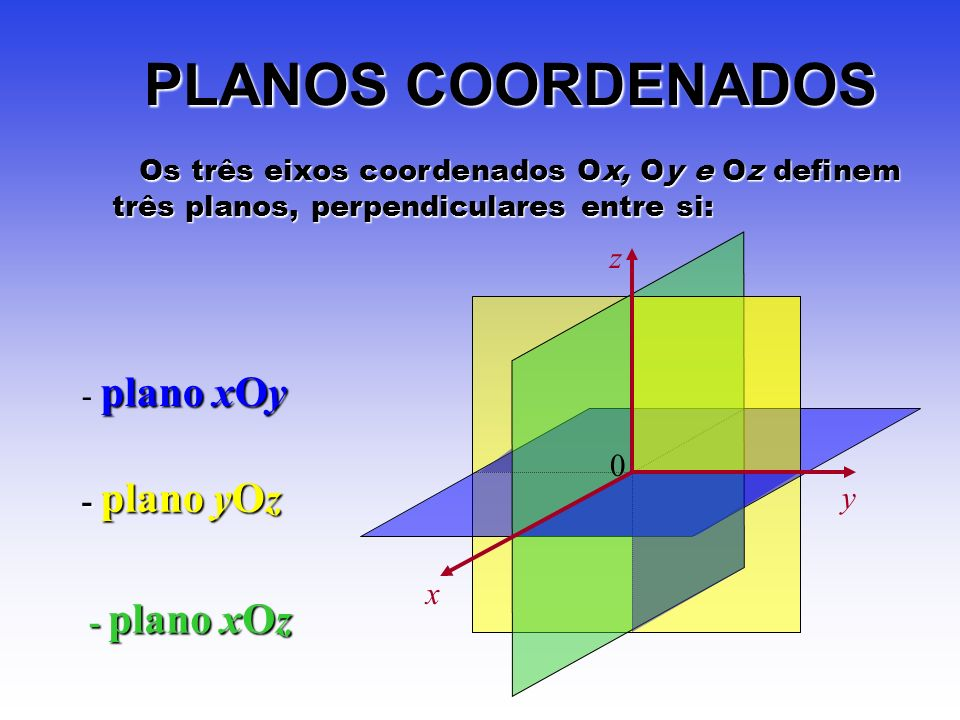
\includegraphics[height=8cm]{images/google-images_planos-coordenados}
			\end{figure}
			%------------------------------
			\tabularnewline
			\midrule
			%------------------------------
			\textbf{Quádricas}
			%------------------------------
			\tabularnewline
			\midrule
			%------------------------------
			\begin{tabular}[c]{@{}c@{}} 

				{\large Quádrica Degenerada (plano)} \\

				{\large $ax + by + cz = 0$} \\
				
			\end{tabular}

			\begin{figure}[H]
                \centering			    
            	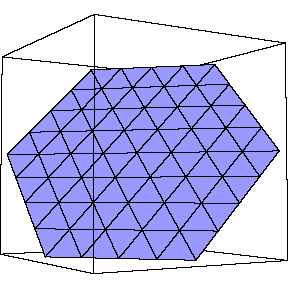
\includegraphics[height=6cm]{images/ufmg_figura-1-3}
			\end{figure}
			%------------------------------
			\tabularnewline
			\midrule
			%------------------------------
			\begin{tabular}[c]{@{}c@{}} 

				{\large Esfera (caso particular do elipsóide)} \\

				{\large $ax^{2} + by^{2} + cz^{2} = k$} \\
				
			\end{tabular}

			\begin{figure}[H]
			    \centering
				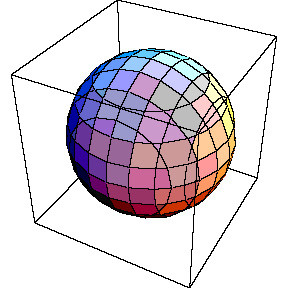
\includegraphics[height=6cm]{images/ufmg_figura-1-1}
			\end{figure}
			%------------------------------
			\tabularnewline
			\midrule
			%------------------------------
			\begin{tabular}[c]{@{}c@{}} 

				{\large Elipsóide} \\

				{\large $ax^{2} + by^{2} + cz^{2} = k$} , ($a \neq b$ ou $b \neq c$ ou $a \neq c$)\\

            \end{tabular}

			\begin{figure}[H]
			    \centering
				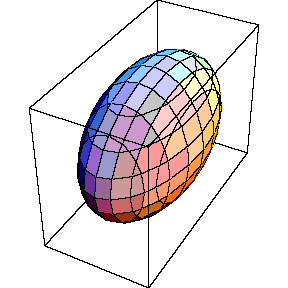
\includegraphics[height=6cm]{images/ufmg_figura-1-2}
			\end{figure}
			%------------------------------
			\tabularnewline
			\midrule
			%------------------------------
			\begin{tabular}[c]{@{}c@{}} 

				{\large Hiperbolóide} \\

				{\large $ax^{2} + by^{2} - cz^{2} = k$} \\

            \end{tabular}

			\begin{figure}[H]
			    \centering	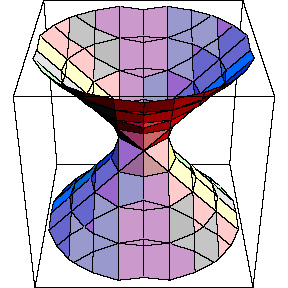
\includegraphics[height=6cm]{images/ufmg_figura-1-4}
			\end{figure}
			%------------------------------
			\tabularnewline
			\midrule
			%------------------------------
			\begin{tabular}[c]{@{}c@{}} 

				{\large Cone} \\

				{\large $ax^{2} + by^{2} - cz^{2} = 0$} \\

            \end{tabular}

			\begin{figure}[H]
			    \centering	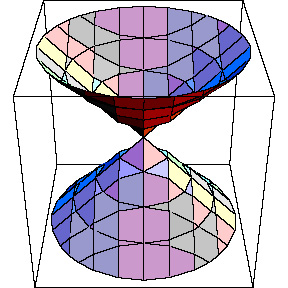
\includegraphics[height=6cm]{images/ufmg_figura-1-5}
			\end{figure}
			%------------------------------
			\tabularnewline
			\midrule
			%------------------------------
			\begin{tabular}[c]{@{}c@{}} 

				{\large Parabolóide} \\

				{\large $ax^{2} + ay^{2} = cz$}\\

            \end{tabular}

			\begin{figure}[H]
			    \centering
				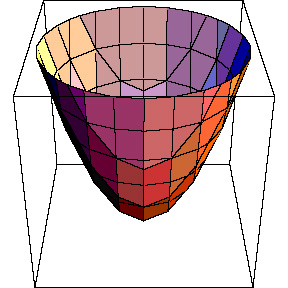
\includegraphics[height=6cm]{images/ufmg_figura-1-6}
			\end{figure}
			%------------------------------
			\tabularnewline
			\midrule
			%------------------------------
			\begin{tabular}[c]{@{}c@{}} 

				{\large Parabolóide Elíptico} \\

				{\large $ax^{2} + by^{2} = cz$}\\

            \end{tabular}

			\begin{figure}[H]
			    \centering
				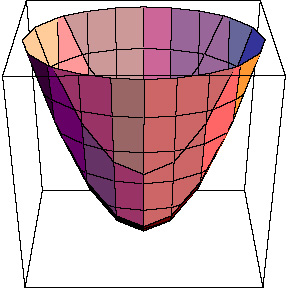
\includegraphics[height=6cm]{images/ufmg_figura-1-7}
			\end{figure}
			%------------------------------
			\tabularnewline
			\midrule
			%------------------------------
			\begin{tabular}[c]{@{}c@{}} 

				{\large Parabolóide Hiperbólico ou Sela} \\

				{\large $ax^{2} - by^{2} = cz$}\\

            \end{tabular}

			\begin{figure}[H]
			    \centering
				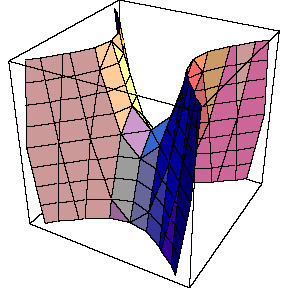
\includegraphics[height=6cm]{images/ufmg_figura-1-8}
			\end{figure}
			%------------------------------
			\tabularnewline
			\midrule
			%------------------------------
			\begin{tabular}[c]{@{}c@{}} 

				{\large Cilindro} \\

				{\large $ax^{2} - by^{2} + dx + ey = k$}\\

            \end{tabular}

			\begin{figure}[H]
			    \centering
				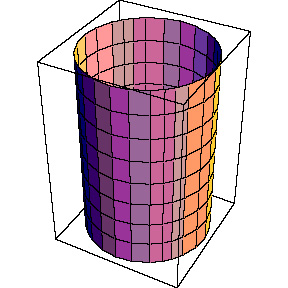
\includegraphics[height=6cm]{images/ufmg_figura-1-9}
			\end{figure}
			%------------------------------
			\tabularnewline
			\bottomrule

		\end{longtable}
		
	\subsection{Derivadas}

		\begin{longtable}{
		@{}
		C{1\textwidth} 
		@{}}

			\toprule
			%------------------------------
			\textbf{Derivadas Parciais}
			%------------------------------
			\tabularnewline
			\midrule
			%------------------------------
			{\large \begin{tabular}[c]{@{}c@{}}

				$\cfrac{\partial f}{\partial x} (x_{0}, y_{0}) = f_{x} = \lim \limits_{\Delta x \to 0} \cfrac{\Delta f}{\Delta x}$ \\

				$\cfrac{\partial f}{\partial y} (x_{0}, y_{0}) = f_{y} = \lim \limits_{\Delta y \to 0} \cfrac{\Delta f}{\Delta y}$

			\end{tabular}}
			%------------------------------
			\tabularnewline
			\midrule
			%------------------------------
			\textbf{Diferencial de uma Função}
			%------------------------------
			\tabularnewline
			\midrule
			%------------------------------
			{\large $df = f_{x} \times \Delta x + f_{y} \times \Delta y$}
			%------------------------------
			\tabularnewline
			\midrule
			%------------------------------
			\textbf{Função Composta - Regra da Cadeia}
			%------------------------------
			\tabularnewline
			\midrule
			%------------------------------
			{\large $\cfrac{dF}{dt} = \cfrac{\partial f}{\partial x} \times \cfrac{dx}{dt} + \cfrac{\partial f}{\partial y} \times \cfrac{dy}{dt}$}
			%------------------------------
			\tabularnewline
			\midrule
			%------------------------------
			\textbf{Derivadas Parciais de Segunda Ordem}
			%------------------------------
			\tabularnewline
			\midrule
			%------------------------------
			{\large \begin{tabular}[c]{@{}c@{}}

				Derivada de $fx$ em relação a $x$ \hspace{1cm} $f_{xx}$ \ ou \ $\cfrac{\partial^{2}f}{\partial x^{2}}$ \\

				Derivada de $fx$ em relação a $y$ \hspace{1cm} $f_{xy}$ \ ou \ $\cfrac{\partial^{2}f}{\partial y\partial x}$ \\

				Derivada de $fy$ em relação a $x$ \hspace{1cm} $f_{yx}$ \ ou \ $\cfrac{\partial^{2}f}{\partial x\partial y}$ \\

				Derivada de $fy$ em relação a $y$ \hspace{1cm} $f_{yy}$ \ ou \ $\cfrac{\partial^{2}f}{\partial y^{2}}$

			\end{tabular}}
			%------------------------------
            \tabularnewline
			\bottomrule

		\end{longtable}

	\subsection{Funções Financeiras/Administrativas}

		\begin{longtable}{
		@{}
		C{1\textwidth} 
		@{}}

			\toprule
			%------------------------------
			\textbf{Função de Cobb-Douglas}
			%------------------------------
			\tabularnewline
			\midrule
			%------------------------------
			{\large $P = f(L, K) = A \times K^{\alpha} \times L^{1 - \alpha}$}
			%------------------------------
			\tabularnewline
			\bottomrule

		\end{longtable}
		
	\subsection{Integrais $(\int)$}

		\begin{longtable}{
		@{}
		C{1\textwidth} 
		@{}}

			\toprule
			%------------------------------
			\textbf{Integrais Parciais}
			%------------------------------
			\tabularnewline
			\midrule
			%------------------------------
			{\large \begin{tabular}[c]{@{}c@{}}

				Integral parcial em relação a $x$ \hspace{1cm} $\int f(x, y) dx$ \\

				Integral parcial em relação a $y$ \hspace{1cm} $\int f(x, y) dy$


			\end{tabular}}
			%------------------------------
			\tabularnewline
			\midrule
			%------------------------------
			\textbf{Integrais Duplas}
			%------------------------------
			\tabularnewline
			\midrule
			%------------------------------
			{\large \begin{tabular}[c]{@{}c@{}}

				$A(x) = \int \limits^{d}_{c} f(x, y)dy$ \hspace{1cm} $V = \int \limits^{b}_{a} A(x)dx$ \\

				$B(y) = \int \limits^{b}_{a} f(x, y)dx$ \hspace{1cm} $V = \int \limits^{d}_{c} B(y)dy$

			\end{tabular}}
			%------------------------------
			\tabularnewline
			\midrule
			%------------------------------
			{\large \begin{tabular}[c]{@{}c@{}}

				$\iint_{D} f(x, y)dxdy = \int \limits^{b}_{a} \left[ \int \limits^{d}_{c} f(x, y)dx \right] dy$ \\

				$\iint_{D} f(x, y)dydx = \int \limits^{d}_{c} \left[ \int \limits^{b}_{a} f(x, y)dy \right] dx$

			\end{tabular}}
			%------------------------------
			\tabularnewline
			\bottomrule

		\end{longtable}

	\subsection{Estudo de Funções de 2 Variáveis}

		\begin{longtable}{
		@{}
		C{1\textwidth} 
		@{}}

			\toprule
			%------------------------------
			\textbf{Pontos Críticos}
			%------------------------------
			\tabularnewline
			\midrule
			%------------------------------			
			{\large $fx(x_{0}, y_{0}) = 0$ e $fy(x_{0}, y_{0}) = 0$}
			%------------------------------
			\tabularnewline
			\midrule
			%------------------------------
			\textbf{Pontos de Máximo ou Mínimo}
			%------------------------------
			\tabularnewline
			\midrule
			%------------------------------
			{\large \begin{tabular}[c]{@{}c@{}}

				$
				H(x_{0}, y_{0}) =
				\begin{vmatrix}

					f_{xx}(x_{0}, y_{0}) & f_{xy}(x_{0}, y_{0}) \\
					f_{yx}(x_{0}, y_{0}) & f_{yy}(x_{0}, y_{0})
					\end{vmatrix}
				$ \\

				$H(x_{0}, y_{0}) > 0$ e $f_{xx}(x_{0}, y_{0}) < 0$ , $(x_{0}, y_{0})$ será ponto de máximo de $f$ \\

				$H(x_{0}, y_{0}) > 0$ e $f_{xx}(x_{0}, y_{0}) > 0$, $(x_{0}, y_{0})$ será ponto de mínimo de $f$ \\

				$H(x_{0}, y_{0}) < 0$ , $(x_{0}, y_{0})$ será ponto de sela de $f$

			\end{tabular}}
			%------------------------------
			\tabularnewline
			\midrule
			%------------------------------
			{\large \begin{tabular}[c]{@{}c@{}}

				\textbf{Máximos e Mínimos Condicionados} \\

				\textbf{Método dos Multiplicadores de Lagrange}

			\end{tabular}}
			%------------------------------
			\tabularnewline
			\midrule
			%------------------------------
			{\large Não se aplica se \hspace{1cm} $\cfrac{\partial \Phi}{\partial x} (x_{0}, y_{0}) = 0$ \ e \ $\cfrac{\partial \Phi}{\partial y} (x_{0}, y_{0}) = 0$}
			%------------------------------
			\tabularnewline
			\midrule
			%------------------------------
			{\large \begin{tabular}[c]{@{}c@{}}

				$F(x, y, \lambda) = f(x, y) - \lambda \times \Phi (x, y)$ \\

				$\cfrac{\partial F}{\partial x} = 0$ \hspace{1cm} $\cfrac{\partial F}{\partial y} = 0$ \hspace{1cm} $\cfrac{\partial F}{\partial \lambda} = 0$

			\end{tabular}}
			%------------------------------
			\tabularnewline
			\midrule
			%------------------------------
			{\large \begin{tabular}[c]{@{}c@{}}

				$\cfrac{\partial f}{\partial x} (x_{0}, y_{0}) = \lambda \times \cfrac{\partial \Phi}{\partial x} (x_{0}, y_{0})$ \hspace{1cm} $\cfrac{\partial f}{\partial y} (x_{0}, y_{0}) = \lambda \times \cfrac{\partial \Phi}{\partial y} (x_{0}, y_{0})$ \\

				$\cfrac{\partial f}{\partial x} = \lambda \times \cfrac{\partial \Phi}{\partial x}$ \hspace{1cm} $\cfrac{\partial f}{\partial y} = \lambda \times \cfrac{\partial \Phi}{\partial y}$ \hspace{1cm} $\Phi (x, y) = 0$

			\end{tabular}}
			%------------------------------
			\tabularnewline
			\bottomrule

		\end{longtable}